\documentclass[1p]{elsarticle_modified}
%\bibliographystyle{elsarticle-num}

%\usepackage[colorlinks]{hyperref}
%\usepackage{abbrmath_seonhwa} %\Abb, \Ascr, \Acal ,\Abf, \Afrak
\usepackage{amsfonts}
\usepackage{amssymb}
\usepackage{amsmath}
\usepackage{amsthm}
\usepackage{scalefnt}
\usepackage{amsbsy}
\usepackage{kotex}
\usepackage{caption}
\usepackage{subfig}
\usepackage{color}
\usepackage{graphicx}
\usepackage{xcolor} %% white, black, red, green, blue, cyan, magenta, yellow
\usepackage{float}
\usepackage{setspace}
\usepackage{hyperref}

\usepackage{tikz}
\usetikzlibrary{arrows}

\usepackage{multirow}
\usepackage{array} % fixed length table
\usepackage{hhline}

%%%%%%%%%%%%%%%%%%%%%
\makeatletter
\renewcommand*\env@matrix[1][\arraystretch]{%
	\edef\arraystretch{#1}%
	\hskip -\arraycolsep
	\let\@ifnextchar\new@ifnextchar
	\array{*\c@MaxMatrixCols c}}
\makeatother %https://tex.stackexchange.com/questions/14071/how-can-i-increase-the-line-spacing-in-a-matrix
%%%%%%%%%%%%%%%

\usepackage[normalem]{ulem}

\newcommand{\msout}[1]{\ifmmode\text{\sout{\ensuremath{#1}}}\else\sout{#1}\fi}
%SOURCE: \msout is \stkout macro in https://tex.stackexchange.com/questions/20609/strikeout-in-math-mode

\newcommand{\cancel}[1]{
	\ifmmode
	{\color{red}\msout{#1}}
	\else
	{\color{red}\sout{#1}}
	\fi
}

\newcommand{\add}[1]{
	{\color{blue}\uwave{#1}}
}

\newcommand{\replace}[2]{
	\ifmmode
	{\color{red}\msout{#1}}{\color{blue}\uwave{#2}}
	\else
	{\color{red}\sout{#1}}{\color{blue}\uwave{#2}}
	\fi
}

\newcommand{\Sol}{\mathcal{S}} %segment
\newcommand{\D}{D} %diagram
\newcommand{\A}{\mathcal{A}} %arc


%%%%%%%%%%%%%%%%%%%%%%%%%%%%%5 test

\def\sl{\operatorname{\textup{SL}}(2,\Cbb)}
\def\psl{\operatorname{\textup{PSL}}(2,\Cbb)}
\def\quan{\mkern 1mu \triangleright \mkern 1mu}

\theoremstyle{definition}
\newtheorem{thm}{Theorem}[section]
\newtheorem{prop}[thm]{Proposition}
\newtheorem{lem}[thm]{Lemma}
\newtheorem{ques}[thm]{Question}
\newtheorem{cor}[thm]{Corollary}
\newtheorem{defn}[thm]{Definition}
\newtheorem{exam}[thm]{Example}
\newtheorem{rmk}[thm]{Remark}
\newtheorem{alg}[thm]{Algorithm}

\newcommand{\I}{\sqrt{-1}}
\begin{document}

%\begin{frontmatter}
%
%\title{Boundary parabolic representations of knots up to 8 crossings}
%
%%% Group authors per affiliation:
%\author{Yunhi Cho} 
%\address{Department of Mathematics, University of Seoul, Seoul, Korea}
%\ead{yhcho@uos.ac.kr}
%
%
%\author{Seonhwa Kim} %\fnref{s_kim}}
%\address{Center for Geometry and Physics, Institute for Basic Science, Pohang, 37673, Korea}
%\ead{ryeona17@ibs.re.kr}
%
%\author{Hyuk Kim}
%\address{Department of Mathematical Sciences, Seoul National University, Seoul 08826, Korea}
%\ead{hyukkim@snu.ac.kr}
%
%\author{Seokbeom Yoon}
%\address{Department of Mathematical Sciences, Seoul National University, Seoul, 08826,  Korea}
%\ead{sbyoon15@snu.ac.kr}
%
%\begin{abstract}
%We find all boundary parabolic representation of knots up to 8 crossings.
%
%\end{abstract}
%\begin{keyword}
%    \MSC[2010] 57M25 
%\end{keyword}
%
%\end{frontmatter}

%\linenumbers
%\tableofcontents
%
\newcommand\colored[1]{\textcolor{white}{\rule[-0.35ex]{0.8em}{1.4ex}}\kern-0.8em\color{red} #1}%
%\newcommand\colored[1]{\textcolor{white}{ #1}\kern-2.17ex	\textcolor{white}{ #1}\kern-1.81ex	\textcolor{white}{ #1}\kern-2.15ex\color{red}#1	}

{\Large $\underline{12n_{0058}~(K12n_{0058})}$}

\setlength{\tabcolsep}{10pt}
\renewcommand{\arraystretch}{1.6}
\vspace{1cm}\begin{tabular}{m{100pt}>{\centering\arraybackslash}m{274pt}}
\multirow{5}{120pt}{
	\centering
	\includegraphics[width=112pt]{../../../GIT/diagram.site/Diagrams/png/2147_12n_0058.png}\\
\ \ \ A knot diagram\footnotemark}&
\allowdisplaybreaks
\textbf{Linearized knot diagam} \\
\cline{2-2}
 &
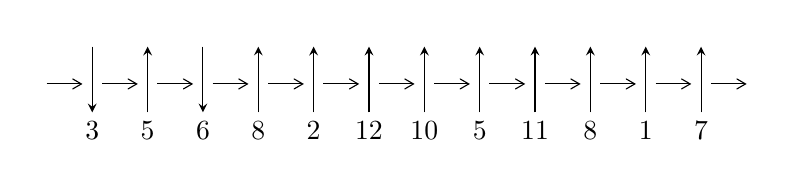
\begin{tikzpicture}[x=20pt, y=17pt]
	% nodes
	\node (C0) at (0, 0) {};
	\node (C1) at (1, 0) {};
	\node (C1U) at (1, +1) {};
	\node (C1D) at (1, -1) {3};

	\node (C2) at (2, 0) {};
	\node (C2U) at (2, +1) {};
	\node (C2D) at (2, -1) {5};

	\node (C3) at (3, 0) {};
	\node (C3U) at (3, +1) {};
	\node (C3D) at (3, -1) {6};

	\node (C4) at (4, 0) {};
	\node (C4U) at (4, +1) {};
	\node (C4D) at (4, -1) {8};

	\node (C5) at (5, 0) {};
	\node (C5U) at (5, +1) {};
	\node (C5D) at (5, -1) {2};

	\node (C6) at (6, 0) {};
	\node (C6U) at (6, +1) {};
	\node (C6D) at (6, -1) {12};

	\node (C7) at (7, 0) {};
	\node (C7U) at (7, +1) {};
	\node (C7D) at (7, -1) {10};

	\node (C8) at (8, 0) {};
	\node (C8U) at (8, +1) {};
	\node (C8D) at (8, -1) {5};

	\node (C9) at (9, 0) {};
	\node (C9U) at (9, +1) {};
	\node (C9D) at (9, -1) {11};

	\node (C10) at (10, 0) {};
	\node (C10U) at (10, +1) {};
	\node (C10D) at (10, -1) {8};

	\node (C11) at (11, 0) {};
	\node (C11U) at (11, +1) {};
	\node (C11D) at (11, -1) {1};

	\node (C12) at (12, 0) {};
	\node (C12U) at (12, +1) {};
	\node (C12D) at (12, -1) {7};
	\node (C13) at (13, 0) {};

	% arrows
	\draw[->,>={angle 60}]
	(C0) edge (C1) (C1) edge (C2) (C2) edge (C3) (C3) edge (C4) (C4) edge (C5) (C5) edge (C6) (C6) edge (C7) (C7) edge (C8) (C8) edge (C9) (C9) edge (C10) (C10) edge (C11) (C11) edge (C12) (C12) edge (C13) ;	\draw[->,>=stealth]
	(C1U) edge (C1D) (C2D) edge (C2U) (C3U) edge (C3D) (C4D) edge (C4U) (C5D) edge (C5U) (C6D) edge (C6U) (C7D) edge (C7U) (C8D) edge (C8U) (C9D) edge (C9U) (C10D) edge (C10U) (C11D) edge (C11U) (C12D) edge (C12U) ;
	\end{tikzpicture} \\
\hhline{~~} \\& 
\textbf{Solving Sequence} \\ \cline{2-2} 
 &
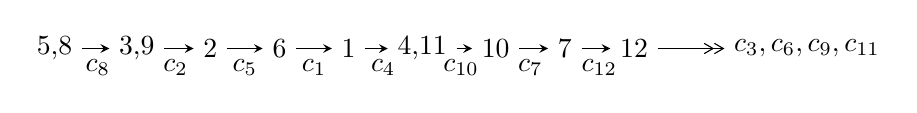
\begin{tikzpicture}[x=25pt, y=7pt]
	% node
	\node (A0) at (-1/8, 0) {5,8};
	\node (A1) at (17/16, 0) {3,9};
	\node (A2) at (17/8, 0) {2};
	\node (A3) at (25/8, 0) {6};
	\node (A4) at (33/8, 0) {1};
	\node (A5) at (83/16, 0) {4,11};
	\node (A6) at (25/4, 0) {10};
	\node (A7) at (29/4, 0) {7};
	\node (A8) at (33/4, 0) {12};
	\node (C1) at (1/2, -1) {$c_{8}$};
	\node (C2) at (13/8, -1) {$c_{2}$};
	\node (C3) at (21/8, -1) {$c_{5}$};
	\node (C4) at (29/8, -1) {$c_{1}$};
	\node (C5) at (37/8, -1) {$c_{4}$};
	\node (C6) at (23/4, -1) {$c_{10}$};
	\node (C7) at (27/4, -1) {$c_{7}$};
	\node (C8) at (31/4, -1) {$c_{12}$};
	\node (A9) at (43/4, 0) {$c_{3},c_{6},c_{9},c_{11}$};

	% edge
	\draw[->,>=stealth]	
	(A0) edge (A1) (A1) edge (A2) (A2) edge (A3) (A3) edge (A4) (A4) edge (A5) (A5) edge (A6) (A6) edge (A7) (A7) edge (A8) ;
	\draw[->>,>={angle 60}]	
	(A8) edge (A9);
\end{tikzpicture} \\ 

\end{tabular} \\

\footnotetext{
The image of knot diagram is generated by the software ``\textbf{Draw programme}" developed by Andrew Bartholomew(\url{http://www.layer8.co.uk/maths/draw/index.htm\#Running-draw}), where we modified some parts for our purpose(\url{https://github.com/CATsTAILs/LinksPainter}).
}\phantom \\ \newline 
\centering \textbf{Ideals for irreducible components\footnotemark of $X_{\text{par}}$} 
 
\begin{align*}
I^u_{1}&=\langle 
6.96435\times10^{33} u^{30}-1.25405\times10^{34} u^{29}+\cdots+1.08242\times10^{37} d+4.63583\times10^{36},\\
\phantom{I^u_{1}}&\phantom{= \langle  }9.28423\times10^{34} u^{30}+2.43126\times10^{35} u^{29}+\cdots+2.16483\times10^{37} c-1.72516\times10^{37},\\
\phantom{I^u_{1}}&\phantom{= \langle  }5.70526\times10^{35} u^{30}+1.13115\times10^{36} u^{29}+\cdots+1.08242\times10^{37} b+2.53478\times10^{37},\\
\phantom{I^u_{1}}&\phantom{= \langle  }-4.91990\times10^{35} u^{30}-1.12026\times10^{36} u^{29}+\cdots+2.16483\times10^{37} a-3.93806\times10^{37},\\
\phantom{I^u_{1}}&\phantom{= \langle  }u^{31}+3 u^{30}+\cdots+64 u+32\rangle \\
I^u_{2}&=\langle 
38636161249 u^{22} c-6684998365 u^{22}+\cdots-212657671098 c+31359529106,\\
\phantom{I^u_{2}}&\phantom{= \langle  }709294494705 u^{22} c-467986206381 u^{22}+\cdots+1120177291630 c+112735730394,\\
\phantom{I^u_{2}}&\phantom{= \langle  }-215916739835 u^{22}+130467973157 u^{21}+\cdots+574976483848 b-314250588698,\\
\phantom{I^u_{2}}&\phantom{= \langle  }-153137520489 u^{22}+68036492975 u^{21}+\cdots+1149952967696 a-806106649958,\\
\phantom{I^u_{2}}&\phantom{= \langle  }u^{23}- u^{22}+\cdots+8 u+4\rangle \\
\\
I^v_{1}&=\langle 
a,\;d,\;c-1,\;b+v,\;v^2- v+1\rangle \\
I^v_{2}&=\langle 
a,\;d+1,\;a v+c- a+1,\;b+v,\;v^2- v+1\rangle \\
I^v_{3}&=\langle 
c,\;d+1,\;b,\;a+1,\;v+1\rangle \\
I^v_{4}&=\langle 
c,\;d+1,\;- v^2 b a+v^3 b- v^2 b+a v- v^2+c,\;b^2 v^2- b v+1\rangle \\
\end{align*}
\raggedright * 5 irreducible components of $\dim_{\mathbb{C}}=0$, with total 82 representations.\\
\raggedright * 1 irreducible components of $\dim_{\mathbb{C}}=1$ \\
\footnotetext{All coefficients of polynomials are rational numbers. But the coefficients are sometimes approximated in decimal forms when there is not enough margin.}
\newpage
\renewcommand{\arraystretch}{1}
\centering \section*{I. $I^u_{1}= \langle 6.96\times10^{33} u^{30}-1.25\times10^{34} u^{29}+\cdots+1.08\times10^{37} d+4.64\times10^{36},\;9.28\times10^{34} u^{30}+2.43\times10^{35} u^{29}+\cdots+2.16\times10^{37} c-1.73\times10^{37},\;5.71\times10^{35} u^{30}+1.13\times10^{36} u^{29}+\cdots+1.08\times10^{37} b+2.53\times10^{37},\;-4.92\times10^{35} u^{30}-1.12\times10^{36} u^{29}+\cdots+2.16\times10^{37} a-3.94\times10^{37},\;u^{31}+3 u^{30}+\cdots+64 u+32 \rangle$}
\flushleft \textbf{(i) Arc colorings}\\
\begin{tabular}{m{7pt} m{180pt} m{7pt} m{180pt} }
\flushright $a_{5}=$&$\begin{pmatrix}0\\u\end{pmatrix}$ \\
\flushright $a_{8}=$&$\begin{pmatrix}1\\0\end{pmatrix}$ \\
\flushright $a_{3}=$&$\begin{pmatrix}0.0227265 u^{30}+0.0517482 u^{29}+\cdots+2.69661 u+1.81911\\-0.0527085 u^{30}-0.104502 u^{29}+\cdots-2.42240 u-2.34178\end{pmatrix}$ \\
\flushright $a_{9}=$&$\begin{pmatrix}1\\- u^2\end{pmatrix}$ \\
\flushright $a_{2}=$&$\begin{pmatrix}0.0227265 u^{30}+0.0517482 u^{29}+\cdots+2.69661 u+1.81911\\-0.0423983 u^{30}-0.0818074 u^{29}+\cdots-2.09805 u-1.81598\end{pmatrix}$ \\
\flushright $a_{6}=$&$\begin{pmatrix}0.0368633 u^{30}+0.0974729 u^{29}+\cdots+0.270429 u+0.869375\\-0.0613442 u^{30}-0.159676 u^{29}+\cdots+0.274410 u-2.98789\end{pmatrix}$ \\
\flushright $a_{1}=$&$\begin{pmatrix}0.0244809 u^{30}+0.0622027 u^{29}+\cdots-0.544839 u+2.11852\\-0.0715195 u^{30}-0.187609 u^{29}+\cdots+0.338443 u-3.34757\end{pmatrix}$ \\
\flushright $a_{4}=$&$\begin{pmatrix}- u\\u\end{pmatrix}$ \\
\flushright $a_{11}=$&$\begin{pmatrix}-0.00428866 u^{30}-0.0112307 u^{29}+\cdots-0.0728208 u+0.796905\\-0.000643408 u^{30}+0.00115856 u^{29}+\cdots+0.160798 u-0.428286\end{pmatrix}$ \\
\flushright $a_{10}=$&$\begin{pmatrix}-0.00364526 u^{30}-0.0123893 u^{29}+\cdots-0.233619 u+1.22519\\-0.000643408 u^{30}+0.00115856 u^{29}+\cdots+0.160798 u-0.428286\end{pmatrix}$ \\
\flushright $a_{7}=$&$\begin{pmatrix}-0.00116998 u^{30}+0.000296647 u^{29}+\cdots+0.120558 u+0.316290\\-0.00311868 u^{30}-0.0115274 u^{29}+\cdots-0.193379 u+0.480614\end{pmatrix}$ \\
\flushright $a_{12}=$&$\begin{pmatrix}0.0281261 u^{30}+0.0745920 u^{29}+\cdots-0.311221 u+1.89333\\-0.0708761 u^{30}-0.188768 u^{29}+\cdots+0.177645 u-2.91928\end{pmatrix}$\\&\end{tabular}
\flushleft \textbf{(ii) Obstruction class $= -1$}\\~\\
\flushleft \textbf{(iii) Cusp Shapes $= 0.0330834 u^{30}+0.0743041 u^{29}+\cdots+9.35750 u+13.8824$}\\~\\
\newpage\renewcommand{\arraystretch}{1}
\flushleft \textbf{(iv) u-Polynomials at the component}\newline \\
\begin{tabular}{m{50pt}|m{274pt}}
Crossings & \hspace{64pt}u-Polynomials at each crossing \\
\hline $$\begin{aligned}c_{1}\end{aligned}$$&$\begin{aligned}
&u^{31}+15 u^{30}+\cdots+120 u-16
\end{aligned}$\\
\hline $$\begin{aligned}c_{2},c_{5}\end{aligned}$$&$\begin{aligned}
&u^{31}+u^{30}+\cdots+8 u-4
\end{aligned}$\\
\hline $$\begin{aligned}c_{3}\end{aligned}$$&$\begin{aligned}
&u^{31}- u^{30}+\cdots+128 u-548
\end{aligned}$\\
\hline $$\begin{aligned}c_{4},c_{8}\end{aligned}$$&$\begin{aligned}
&u^{31}-3 u^{30}+\cdots+64 u-32
\end{aligned}$\\
\hline $$\begin{aligned}c_{6},c_{7},c_{10}\\c_{12}\end{aligned}$$&$\begin{aligned}
&u^{31}+5 u^{30}+\cdots-3 u-1
\end{aligned}$\\
\hline $$\begin{aligned}c_{9},c_{11}\end{aligned}$$&$\begin{aligned}
&u^{31}-11 u^{30}+\cdots+21 u-1
\end{aligned}$\\
\hline
\end{tabular}\\~\\
\newpage\renewcommand{\arraystretch}{1}
\flushleft \textbf{(v) Riley Polynomials at the component}\newline \\
\begin{tabular}{m{50pt}|m{274pt}}
Crossings & \hspace{64pt}Riley Polynomials at each crossing \\
\hline $$\begin{aligned}c_{1}\end{aligned}$$&$\begin{aligned}
&y^{31}+3 y^{30}+\cdots+25888 y-256
\end{aligned}$\\
\hline $$\begin{aligned}c_{2},c_{5}\end{aligned}$$&$\begin{aligned}
&y^{31}+15 y^{30}+\cdots+120 y-16
\end{aligned}$\\
\hline $$\begin{aligned}c_{3}\end{aligned}$$&$\begin{aligned}
&y^{31}-9 y^{30}+\cdots+4451896 y-300304
\end{aligned}$\\
\hline $$\begin{aligned}c_{4},c_{8}\end{aligned}$$&$\begin{aligned}
&y^{31}+15 y^{30}+\cdots+1024 y-1024
\end{aligned}$\\
\hline $$\begin{aligned}c_{6},c_{7},c_{10}\\c_{12}\end{aligned}$$&$\begin{aligned}
&y^{31}-11 y^{30}+\cdots+21 y-1
\end{aligned}$\\
\hline $$\begin{aligned}c_{9},c_{11}\end{aligned}$$&$\begin{aligned}
&y^{31}+29 y^{30}+\cdots+61 y-1
\end{aligned}$\\
\hline
\end{tabular}\\~\\
\newpage\flushleft \textbf{(vi) Complex Volumes and Cusp Shapes}
$$\begin{array}{c|c|c}  
\text{Solutions to }I^u_{1}& \I (\text{vol} + \sqrt{-1}CS) & \text{Cusp shape}\\
 \hline 
\begin{aligned}
u &= \phantom{-}0.753219 + 0.379837 I \\
a &= -0.743282 - 0.874244 I \\
b &= \phantom{-}0.716703 + 0.640811 I \\
c &= \phantom{-}0.685053 - 0.287784 I \\
d &= -0.240774 - 0.521238 I\end{aligned}
 & -1.42006 + 1.96537 I & \phantom{-}1.93692 - 5.44006 I \\ \hline\begin{aligned}
u &= \phantom{-}0.753219 - 0.379837 I \\
a &= -0.743282 + 0.874244 I \\
b &= \phantom{-}0.716703 - 0.640811 I \\
c &= \phantom{-}0.685053 + 0.287784 I \\
d &= -0.240774 + 0.521238 I\end{aligned}
 & -1.42006 - 1.96537 I & \phantom{-}1.93692 + 5.44006 I \\ \hline\begin{aligned}
u &= -0.337564 + 1.132290 I \\
a &= -0.588580 + 0.817543 I \\
b &= -1.10048 + 1.34389 I \\
c &= \phantom{-}0.17117 - 1.61585 I \\
d &= \phantom{-}0.935169 - 0.612003 I\end{aligned}
 & \phantom{-}0.45247 - 2.02679 I & \phantom{-}7.73031 + 3.42583 I \\ \hline\begin{aligned}
u &= -0.337564 - 1.132290 I \\
a &= -0.588580 - 0.817543 I \\
b &= -1.10048 - 1.34389 I \\
c &= \phantom{-}0.17117 + 1.61585 I \\
d &= \phantom{-}0.935169 + 0.612003 I\end{aligned}
 & \phantom{-}0.45247 + 2.02679 I & \phantom{-}7.73031 - 3.42583 I \\ \hline\begin{aligned}
u &= \phantom{-}1.121020 + 0.424146 I \\
a &= -0.661458 + 0.037458 I \\
b &= \phantom{-}1.62605 + 0.80238 I \\
c &= \phantom{-}0.460731 + 0.138106 I \\
d &= -0.991521 + 0.596969 I\end{aligned}
 & \phantom{-}1.55877 - 4.66712 I & \phantom{-}11.51750 + 4.56967 I \\ \hline\begin{aligned}
u &= \phantom{-}1.121020 - 0.424146 I \\
a &= -0.661458 - 0.037458 I \\
b &= \phantom{-}1.62605 - 0.80238 I \\
c &= \phantom{-}0.460731 - 0.138106 I \\
d &= -0.991521 - 0.596969 I\end{aligned}
 & \phantom{-}1.55877 + 4.66712 I & \phantom{-}11.51750 - 4.56967 I\\
 \hline 
 \end{array}$$\newpage$$\begin{array}{c|c|c}  
\text{Solutions to }I^u_{1}& \I (\text{vol} + \sqrt{-1}CS) & \text{Cusp shape}\\
 \hline 
\begin{aligned}
u &= \phantom{-}0.698083 + 0.364692 I \\
a &= \phantom{-}0.272982 - 1.147330 I \\
b &= -1.63704 + 2.06806 I \\
c &= \phantom{-}0.498679 + 0.078631 I \\
d &= -0.956651 + 0.308522 I\end{aligned}
 & \phantom{-}3.68376 - 3.19069 I & \phantom{-}14.6846 + 5.1485 I \\ \hline\begin{aligned}
u &= \phantom{-}0.698083 - 0.364692 I \\
a &= \phantom{-}0.272982 + 1.147330 I \\
b &= -1.63704 - 2.06806 I \\
c &= \phantom{-}0.498679 - 0.078631 I \\
d &= -0.956651 - 0.308522 I\end{aligned}
 & \phantom{-}3.68376 + 3.19069 I & \phantom{-}14.6846 - 5.1485 I \\ \hline\begin{aligned}
u &= -1.235540 + 0.189024 I \\
a &= \phantom{-}0.397076 - 0.873318 I \\
b &= -1.100320 + 0.790305 I \\
c &= \phantom{-}0.472913 - 0.179552 I \\
d &= -0.848142 - 0.701686 I\end{aligned}
 & -2.56816 + 1.34649 I & \phantom{-}5.38369 - 2.07194 I \\ \hline\begin{aligned}
u &= -1.235540 - 0.189024 I \\
a &= \phantom{-}0.397076 + 0.873318 I \\
b &= -1.100320 - 0.790305 I \\
c &= \phantom{-}0.472913 + 0.179552 I \\
d &= -0.848142 + 0.701686 I\end{aligned}
 & -2.56816 - 1.34649 I & \phantom{-}5.38369 + 2.07194 I \\ \hline\begin{aligned}
u &= \phantom{-}0.464557 + 1.163760 I \\
a &= -0.762353 + 0.385358 I \\
b &= \phantom{-}0.17520 + 1.91640 I \\
c &= -0.05406 + 1.60814 I \\
d &= \phantom{-}1.020880 + 0.621136 I\end{aligned}
 & \phantom{-}1.15318 + 7.72517 I & \phantom{-}9.61403 - 8.29170 I \\ \hline\begin{aligned}
u &= \phantom{-}0.464557 - 1.163760 I \\
a &= -0.762353 - 0.385358 I \\
b &= \phantom{-}0.17520 - 1.91640 I \\
c &= -0.05406 - 1.60814 I \\
d &= \phantom{-}1.020880 - 0.621136 I\end{aligned}
 & \phantom{-}1.15318 - 7.72517 I & \phantom{-}9.61403 + 8.29170 I\\
 \hline 
 \end{array}$$\newpage$$\begin{array}{c|c|c}  
\text{Solutions to }I^u_{1}& \I (\text{vol} + \sqrt{-1}CS) & \text{Cusp shape}\\
 \hline 
\begin{aligned}
u &= -1.253240 + 0.506936 I \\
a &= \phantom{-}0.045977 + 0.940408 I \\
b &= -1.72925 - 0.22350 I \\
c &= \phantom{-}0.439439 - 0.143874 I \\
d &= -1.055310 - 0.672917 I\end{aligned}
 & -1.12377 + 9.51847 I & \phantom{-}8.01541 - 7.69926 I \\ \hline\begin{aligned}
u &= -1.253240 - 0.506936 I \\
a &= \phantom{-}0.045977 - 0.940408 I \\
b &= -1.72925 + 0.22350 I \\
c &= \phantom{-}0.439439 + 0.143874 I \\
d &= -1.055310 + 0.672917 I\end{aligned}
 & -1.12377 - 9.51847 I & \phantom{-}8.01541 + 7.69926 I \\ \hline\begin{aligned}
u &= \phantom{-}0.223678 + 1.371700 I \\
a &= \phantom{-}0.023144 - 0.618799 I \\
b &= -0.490393 - 0.901482 I \\
c &= \phantom{-}0.413752 - 0.939419 I \\
d &= \phantom{-}0.607334 - 0.891545 I\end{aligned}
 & -4.93468 - 0.57606 I & \phantom{-}5.79676 + 1.97891 I \\ \hline\begin{aligned}
u &= \phantom{-}0.223678 - 1.371700 I \\
a &= \phantom{-}0.023144 + 0.618799 I \\
b &= -0.490393 + 0.901482 I \\
c &= \phantom{-}0.413752 + 0.939419 I \\
d &= \phantom{-}0.607334 + 0.891545 I\end{aligned}
 & -4.93468 + 0.57606 I & \phantom{-}5.79676 - 1.97891 I \\ \hline\begin{aligned}
u &= -0.591801\phantom{ +0.000000I} \\
a &= \phantom{-}0.533366\phantom{ +0.000000I} \\
b &= -0.736939\phantom{ +0.000000I} \\
c &= \phantom{-}0.699591\phantom{ +0.000000I} \\
d &= -0.429406\phantom{ +0.000000I}\end{aligned}
 & \phantom{-}0.834149\phantom{ +0.000000I} & \phantom{-}11.9720\phantom{ +0.000000I} \\ \hline\begin{aligned}
u &= -0.540907 + 0.236782 I \\
a &= -1.50466 + 1.00061 I \\
b &= \phantom{-}3.58655 - 2.56486 I \\
c &= \phantom{-}0.518602 - 0.047373 I \\
d &= -0.912302 - 0.174686 I\end{aligned}
 & \phantom{-}3.12062 - 1.49349 I & \phantom{-}14.4230 + 1.8126 I\\
 \hline 
 \end{array}$$\newpage$$\begin{array}{c|c|c}  
\text{Solutions to }I^u_{1}& \I (\text{vol} + \sqrt{-1}CS) & \text{Cusp shape}\\
 \hline 
\begin{aligned}
u &= -0.540907 - 0.236782 I \\
a &= -1.50466 - 1.00061 I \\
b &= \phantom{-}3.58655 + 2.56486 I \\
c &= \phantom{-}0.518602 + 0.047373 I \\
d &= -0.912302 + 0.174686 I\end{aligned}
 & \phantom{-}3.12062 + 1.49349 I & \phantom{-}14.4230 - 1.8126 I \\ \hline\begin{aligned}
u &= \phantom{-}0.067118 + 0.557682 I \\
a &= \phantom{-}1.39023 + 1.20733 I \\
b &= \phantom{-}0.343697 + 0.692018 I \\
c &= \phantom{-}1.45537 - 0.23813 I \\
d &= \phantom{-}0.330807 - 0.109496 I\end{aligned}
 & \phantom{-}0.46111 - 2.29513 I & \phantom{-}1.47827 + 3.85950 I \\ \hline\begin{aligned}
u &= \phantom{-}0.067118 - 0.557682 I \\
a &= \phantom{-}1.39023 - 1.20733 I \\
b &= \phantom{-}0.343697 - 0.692018 I \\
c &= \phantom{-}1.45537 + 0.23813 I \\
d &= \phantom{-}0.330807 + 0.109496 I\end{aligned}
 & \phantom{-}0.46111 + 2.29513 I & \phantom{-}1.47827 - 3.85950 I \\ \hline\begin{aligned}
u &= \phantom{-}0.71578 + 1.28059 I \\
a &= \phantom{-}0.097632 - 0.639247 I \\
b &= -1.59966 - 0.59378 I \\
c &= -0.37486 + 1.39000 I \\
d &= \phantom{-}1.180860 + 0.670647 I\end{aligned}
 & -1.16605 + 11.32090 I & \phantom{-}10.43454 - 6.71502 I \\ \hline\begin{aligned}
u &= \phantom{-}0.71578 - 1.28059 I \\
a &= \phantom{-}0.097632 + 0.639247 I \\
b &= -1.59966 + 0.59378 I \\
c &= -0.37486 - 1.39000 I \\
d &= \phantom{-}1.180860 - 0.670647 I\end{aligned}
 & -1.16605 - 11.32090 I & \phantom{-}10.43454 + 6.71502 I \\ \hline\begin{aligned}
u &= -0.39077 + 1.46203 I \\
a &= -0.858408 - 0.114457 I \\
b &= \phantom{-}1.17073 - 1.58917 I \\
c &= \phantom{-}0.382686 + 0.821951 I \\
d &= \phantom{-}0.534475 + 0.999877 I\end{aligned}
 & -8.24554 - 4.31764 I & \phantom{-}2.71892 + 1.88458 I\\
 \hline 
 \end{array}$$\newpage$$\begin{array}{c|c|c}  
\text{Solutions to }I^u_{1}& \I (\text{vol} + \sqrt{-1}CS) & \text{Cusp shape}\\
 \hline 
\begin{aligned}
u &= -0.39077 - 1.46203 I \\
a &= -0.858408 + 0.114457 I \\
b &= \phantom{-}1.17073 + 1.58917 I \\
c &= \phantom{-}0.382686 - 0.821951 I \\
d &= \phantom{-}0.534475 - 0.999877 I\end{aligned}
 & -8.24554 + 4.31764 I & \phantom{-}2.71892 - 1.88458 I \\ \hline\begin{aligned}
u &= -0.79393 + 1.30401 I \\
a &= -0.862730 + 0.059745 I \\
b &= \phantom{-}1.76369 - 2.19058 I \\
c &= -0.444220 - 1.327190 I \\
d &= \phantom{-}1.226790 - 0.677567 I\end{aligned}
 & -3.7041 - 16.8176 I & \phantom{-}8.02968 + 10.05725 I \\ \hline\begin{aligned}
u &= -0.79393 - 1.30401 I \\
a &= -0.862730 - 0.059745 I \\
b &= \phantom{-}1.76369 + 2.19058 I \\
c &= -0.444220 + 1.327190 I \\
d &= \phantom{-}1.226790 + 0.677567 I\end{aligned}
 & -3.7041 + 16.8176 I & \phantom{-}8.02968 - 10.05725 I \\ \hline\begin{aligned}
u &= -0.62073 + 1.40356 I \\
a &= \phantom{-}0.693155 - 0.448111 I \\
b &= -0.266136 + 0.105825 I \\
c &= -0.237422 - 1.289560 I \\
d &= \phantom{-}1.138090 - 0.750034 I\end{aligned}
 & -6.51517 - 8.00123 I & \phantom{-}4.81025 + 4.92455 I \\ \hline\begin{aligned}
u &= -0.62073 - 1.40356 I \\
a &= \phantom{-}0.693155 + 0.448111 I \\
b &= -0.266136 - 0.105825 I \\
c &= -0.237422 + 1.289560 I \\
d &= \phantom{-}1.138090 + 0.750034 I\end{aligned}
 & -6.51517 + 8.00123 I & \phantom{-}4.81025 - 4.92455 I \\ \hline\begin{aligned}
u &= -0.07489 + 1.53753 I \\
a &= \phantom{-}0.794591 - 0.282968 I \\
b &= -0.590866 - 0.831603 I \\
c &= \phantom{-}0.262372 + 0.979829 I \\
d &= \phantom{-}0.744999 + 0.952303 I\end{aligned}
 & -9.13328 + 4.81435 I & \phantom{-}2.44035 - 4.85668 I\\
 \hline 
 \end{array}$$\newpage$$\begin{array}{c|c|c}  
\text{Solutions to }I^u_{1}& \I (\text{vol} + \sqrt{-1}CS) & \text{Cusp shape}\\
 \hline 
\begin{aligned}
u &= -0.07489 - 1.53753 I \\
a &= \phantom{-}0.794591 + 0.282968 I \\
b &= -0.590866 + 0.831603 I \\
c &= \phantom{-}0.262372 - 0.979829 I \\
d &= \phantom{-}0.744999 - 0.952303 I\end{aligned}
 & -9.13328 - 4.81435 I & \phantom{-}2.44035 + 4.85668 I\\
 \hline 
 \end{array}$$\newpage\newpage\renewcommand{\arraystretch}{1}
\centering \section*{II. $I^u_{2}= \langle 3.86\times10^{10} c u^{22}-6.68\times10^{9} u^{22}+\cdots-2.13\times10^{11} c+3.14\times10^{10},\;7.09\times10^{11} c u^{22}-4.68\times10^{11} u^{22}+\cdots+1.12\times10^{12} c+1.13\times10^{11},\;-2.16\times10^{11} u^{22}+1.30\times10^{11} u^{21}+\cdots+5.75\times10^{11} b-3.14\times10^{11},\;-1.53\times10^{11} u^{22}+6.80\times10^{10} u^{21}+\cdots+1.15\times10^{12} a-8.06\times10^{11},\;u^{23}- u^{22}+\cdots+8 u+4 \rangle$}
\flushleft \textbf{(i) Arc colorings}\\
\begin{tabular}{m{7pt} m{180pt} m{7pt} m{180pt} }
\flushright $a_{5}=$&$\begin{pmatrix}0\\u\end{pmatrix}$ \\
\flushright $a_{8}=$&$\begin{pmatrix}1\\0\end{pmatrix}$ \\
\flushright $a_{3}=$&$\begin{pmatrix}0.133169 u^{22}-0.0591646 u^{21}+\cdots+1.14807 u+0.700991\\0.375523 u^{22}-0.226910 u^{21}+\cdots+3.58831 u+0.546545\end{pmatrix}$ \\
\flushright $a_{9}=$&$\begin{pmatrix}1\\- u^2\end{pmatrix}$ \\
\flushright $a_{2}=$&$\begin{pmatrix}0.133169 u^{22}-0.0591646 u^{21}+\cdots+1.14807 u+0.700991\\0.293213 u^{22}-0.236878 u^{21}+\cdots+2.46360 u+0.250529\end{pmatrix}$ \\
\flushright $a_{6}=$&$\begin{pmatrix}0.0322985 u^{22}-0.252479 u^{21}+\cdots-0.902295 u+0.301575\\0.188074 u^{22}-0.335831 u^{21}+\cdots+0.0919786 u-0.580833\end{pmatrix}$ \\
\flushright $a_{1}=$&$\begin{pmatrix}-0.220372 u^{22}+0.588310 u^{21}+\cdots+0.810316 u+0.279258\\0.0232531 u^{22}+0.239196 u^{21}+\cdots+2.15399 u+0.890919\end{pmatrix}$ \\
\flushright $a_{4}=$&$\begin{pmatrix}- u\\u\end{pmatrix}$ \\
\flushright $a_{11}=$&$\begin{pmatrix}c\\-0.134392 c u^{22}+0.0232531 u^{22}+\cdots+0.739709 c-0.109081\end{pmatrix}$ \\
\flushright $a_{10}=$&$\begin{pmatrix}0.134392 c u^{22}-0.0232531 u^{22}+\cdots+0.260291 c+0.109081\\-0.134392 c u^{22}+0.0232531 u^{22}+\cdots+0.739709 c-0.109081\end{pmatrix}$ \\
\flushright $a_{7}=$&$\begin{pmatrix}-0.134392 c u^{22}+0.0232531 u^{22}+\cdots+1.73971 c-0.109081\\0.134392 c u^{22}-0.0232531 u^{22}+\cdots-0.739709 c+0.109081\end{pmatrix}$ \\
\flushright $a_{12}=$&$\begin{pmatrix}0.0536818 c u^{22}-0.109233 u^{22}+\cdots+1.15888 c-1.35137\\-0.0769349 c u^{22}-0.0878859 u^{22}+\cdots-1.04979 c+1.52155\end{pmatrix}$\\&\end{tabular}
\flushleft \textbf{(ii) Obstruction class $= -1$}\\~\\
\flushleft \textbf{(iii) Cusp Shapes $= \frac{173371509589}{143744120962} u^{22}-\frac{241902270957}{143744120962} u^{21}+\cdots-\frac{379864412243}{143744120962} u+\frac{545150434432}{71872060481}$}\\~\\
\newpage\renewcommand{\arraystretch}{1}
\flushleft \textbf{(iv) u-Polynomials at the component}\newline \\
\begin{tabular}{m{50pt}|m{274pt}}
Crossings & \hspace{64pt}u-Polynomials at each crossing \\
\hline $$\begin{aligned}c_{1}\end{aligned}$$&$\begin{aligned}
&(u^{23}+12 u^{22}+\cdots-2 u-1)^{2}
\end{aligned}$\\
\hline $$\begin{aligned}c_{2},c_{5}\end{aligned}$$&$\begin{aligned}
&(u^{23}+2 u^{22}+\cdots-2 u-1)^{2}
\end{aligned}$\\
\hline $$\begin{aligned}c_{3}\end{aligned}$$&$\begin{aligned}
&(u^{23}-2 u^{22}+\cdots+18 u-9)^{2}
\end{aligned}$\\
\hline $$\begin{aligned}c_{4},c_{8}\end{aligned}$$&$\begin{aligned}
&(u^{23}+u^{22}+\cdots+8 u-4)^{2}
\end{aligned}$\\
\hline $$\begin{aligned}c_{6},c_{7},c_{10}\\c_{12}\end{aligned}$$&$\begin{aligned}
&u^{46}+3 u^{45}+\cdots+56 u+16
\end{aligned}$\\
\hline $$\begin{aligned}c_{9},c_{11}\end{aligned}$$&$\begin{aligned}
&u^{46}-23 u^{45}+\cdots-288 u+256
\end{aligned}$\\
\hline
\end{tabular}\\~\\
\newpage\renewcommand{\arraystretch}{1}
\flushleft \textbf{(v) Riley Polynomials at the component}\newline \\
\begin{tabular}{m{50pt}|m{274pt}}
Crossings & \hspace{64pt}Riley Polynomials at each crossing \\
\hline $$\begin{aligned}c_{1}\end{aligned}$$&$\begin{aligned}
&(y^{23}+24 y^{21}+\cdots+10 y-1)^{2}
\end{aligned}$\\
\hline $$\begin{aligned}c_{2},c_{5}\end{aligned}$$&$\begin{aligned}
&(y^{23}+12 y^{22}+\cdots-2 y-1)^{2}
\end{aligned}$\\
\hline $$\begin{aligned}c_{3}\end{aligned}$$&$\begin{aligned}
&(y^{23}-12 y^{22}+\cdots-450 y-81)^{2}
\end{aligned}$\\
\hline $$\begin{aligned}c_{4},c_{8}\end{aligned}$$&$\begin{aligned}
&(y^{23}+15 y^{22}+\cdots-40 y-16)^{2}
\end{aligned}$\\
\hline $$\begin{aligned}c_{6},c_{7},c_{10}\\c_{12}\end{aligned}$$&$\begin{aligned}
&y^{46}-23 y^{45}+\cdots-288 y+256
\end{aligned}$\\
\hline $$\begin{aligned}c_{9},c_{11}\end{aligned}$$&$\begin{aligned}
&y^{46}-3 y^{45}+\cdots-2449920 y+65536
\end{aligned}$\\
\hline
\end{tabular}\\~\\
\newpage\flushleft \textbf{(vi) Complex Volumes and Cusp Shapes}
$$\begin{array}{c|c|c}  
\text{Solutions to }I^u_{2}& \I (\text{vol} + \sqrt{-1}CS) & \text{Cusp shape}\\
 \hline 
\begin{aligned}
u &= -0.969482\phantom{ +0.000000I} \\
a &= \phantom{-}0.635915\phantom{ +0.000000I} \\
b &= -1.38262\phantom{ +0.000000I} \\
c &= \phantom{-}0.546696 + 0.177229 I \\
d &= -0.655217 + 0.536590 I\end{aligned}
 & \phantom{-}0.502753\phantom{ +0.000000I} & \phantom{-}9.67610\phantom{ +0.000000I} \\ \hline\begin{aligned}
u &= -0.969482\phantom{ +0.000000I} \\
a &= \phantom{-}0.635915\phantom{ +0.000000I} \\
b &= -1.38262\phantom{ +0.000000I} \\
c &= \phantom{-}0.546696 - 0.177229 I \\
d &= -0.655217 - 0.536590 I\end{aligned}
 & \phantom{-}0.502753\phantom{ +0.000000I} & \phantom{-}9.67610\phantom{ +0.000000I} \\ \hline\begin{aligned}
u &= \phantom{-}0.308169 + 0.985429 I \\
a &= \phantom{-}0.004284 - 0.666189 I \\
b &= -0.572740 - 0.057611 I \\
c &= \phantom{-}0.430219 + 0.027076 I \\
d &= -1.315230 + 0.145711 I\end{aligned}
 & \phantom{-}2.62555 + 2.00215 I & \phantom{-}10.76412 - 3.62705 I \\ \hline\begin{aligned}
u &= \phantom{-}0.308169 + 0.985429 I \\
a &= \phantom{-}0.004284 - 0.666189 I \\
b &= -0.572740 - 0.057611 I \\
c &= \phantom{-}0.35592 + 1.88659 I \\
d &= \phantom{-}0.903437 + 0.511840 I\end{aligned}
 & \phantom{-}2.62555 + 2.00215 I & \phantom{-}10.76412 - 3.62705 I \\ \hline\begin{aligned}
u &= \phantom{-}0.308169 - 0.985429 I \\
a &= \phantom{-}0.004284 + 0.666189 I \\
b &= -0.572740 + 0.057611 I \\
c &= \phantom{-}0.430219 - 0.027076 I \\
d &= -1.315230 - 0.145711 I\end{aligned}
 & \phantom{-}2.62555 - 2.00215 I & \phantom{-}10.76412 + 3.62705 I \\ \hline\begin{aligned}
u &= \phantom{-}0.308169 - 0.985429 I \\
a &= \phantom{-}0.004284 + 0.666189 I \\
b &= -0.572740 + 0.057611 I \\
c &= \phantom{-}0.35592 - 1.88659 I \\
d &= \phantom{-}0.903437 - 0.511840 I\end{aligned}
 & \phantom{-}2.62555 - 2.00215 I & \phantom{-}10.76412 + 3.62705 I\\
 \hline 
 \end{array}$$\newpage$$\begin{array}{c|c|c}  
\text{Solutions to }I^u_{2}& \I (\text{vol} + \sqrt{-1}CS) & \text{Cusp shape}\\
 \hline 
\begin{aligned}
u &= -0.107498 + 1.054050 I \\
a &= \phantom{-}0.832680 + 0.608094 I \\
b &= \phantom{-}0.35976 + 1.52792 I \\
c &= \phantom{-}0.716893 + 1.112390 I \\
d &= \phantom{-}0.590662 + 0.635162 I\end{aligned}
 & -0.12065 - 2.74438 I & \phantom{-}5.99863 + 3.42075 I \\ \hline\begin{aligned}
u &= -0.107498 + 1.054050 I \\
a &= \phantom{-}0.832680 + 0.608094 I \\
b &= \phantom{-}0.35976 + 1.52792 I \\
c &= \phantom{-}0.60269 - 1.46286 I \\
d &= \phantom{-}0.759232 - 0.584397 I\end{aligned}
 & -0.12065 - 2.74438 I & \phantom{-}5.99863 + 3.42075 I \\ \hline\begin{aligned}
u &= -0.107498 - 1.054050 I \\
a &= \phantom{-}0.832680 - 0.608094 I \\
b &= \phantom{-}0.35976 - 1.52792 I \\
c &= \phantom{-}0.716893 - 1.112390 I \\
d &= \phantom{-}0.590662 - 0.635162 I\end{aligned}
 & -0.12065 + 2.74438 I & \phantom{-}5.99863 - 3.42075 I \\ \hline\begin{aligned}
u &= -0.107498 - 1.054050 I \\
a &= \phantom{-}0.832680 - 0.608094 I \\
b &= \phantom{-}0.35976 - 1.52792 I \\
c &= \phantom{-}0.60269 + 1.46286 I \\
d &= \phantom{-}0.759232 + 0.584397 I\end{aligned}
 & -0.12065 + 2.74438 I & \phantom{-}5.99863 - 3.42075 I \\ \hline\begin{aligned}
u &= -0.000983 + 1.149400 I \\
a &= \phantom{-}0.974897 - 0.337516 I \\
b &= -1.35698 - 0.51540 I \\
c &= \phantom{-}0.547631 - 1.231120 I \\
d &= \phantom{-}0.698366 - 0.678096 I\end{aligned}
 & -0.86138 + 1.33135 I & \phantom{-}4.84050 - 0.67575 I \\ \hline\begin{aligned}
u &= -0.000983 + 1.149400 I \\
a &= \phantom{-}0.974897 - 0.337516 I \\
b &= -1.35698 - 0.51540 I \\
c &= \phantom{-}0.417486 - 0.000081 I \\
d &= -1.395290 - 0.000467 I\end{aligned}
 & -0.86138 + 1.33135 I & \phantom{-}4.84050 - 0.67575 I\\
 \hline 
 \end{array}$$\newpage$$\begin{array}{c|c|c}  
\text{Solutions to }I^u_{2}& \I (\text{vol} + \sqrt{-1}CS) & \text{Cusp shape}\\
 \hline 
\begin{aligned}
u &= -0.000983 - 1.149400 I \\
a &= \phantom{-}0.974897 + 0.337516 I \\
b &= -1.35698 + 0.51540 I \\
c &= \phantom{-}0.547631 + 1.231120 I \\
d &= \phantom{-}0.698366 + 0.678096 I\end{aligned}
 & -0.86138 - 1.33135 I & \phantom{-}4.84050 + 0.67575 I \\ \hline\begin{aligned}
u &= -0.000983 - 1.149400 I \\
a &= \phantom{-}0.974897 + 0.337516 I \\
b &= -1.35698 + 0.51540 I \\
c &= \phantom{-}0.417486 + 0.000081 I \\
d &= -1.395290 + 0.000467 I\end{aligned}
 & -0.86138 - 1.33135 I & \phantom{-}4.84050 + 0.67575 I \\ \hline\begin{aligned}
u &= \phantom{-}1.222080 + 0.199525 I \\
a &= -0.209050 + 0.970065 I \\
b &= \phantom{-}1.41696 - 0.48835 I \\
c &= \phantom{-}0.508002 - 0.253270 I \\
d &= -0.576609 - 0.786036 I\end{aligned}
 & -2.55344 - 3.99588 I & \phantom{-}5.39099 + 3.49800 I \\ \hline\begin{aligned}
u &= \phantom{-}1.222080 + 0.199525 I \\
a &= -0.209050 + 0.970065 I \\
b &= \phantom{-}1.41696 - 0.48835 I \\
c &= \phantom{-}0.473795 + 0.176635 I \\
d &= -0.853067 + 0.690841 I\end{aligned}
 & -2.55344 - 3.99588 I & \phantom{-}5.39099 + 3.49800 I \\ \hline\begin{aligned}
u &= \phantom{-}1.222080 - 0.199525 I \\
a &= -0.209050 - 0.970065 I \\
b &= \phantom{-}1.41696 + 0.48835 I \\
c &= \phantom{-}0.508002 + 0.253270 I \\
d &= -0.576609 + 0.786036 I\end{aligned}
 & -2.55344 + 3.99588 I & \phantom{-}5.39099 - 3.49800 I \\ \hline\begin{aligned}
u &= \phantom{-}1.222080 - 0.199525 I \\
a &= -0.209050 - 0.970065 I \\
b &= \phantom{-}1.41696 + 0.48835 I \\
c &= \phantom{-}0.473795 - 0.176635 I \\
d &= -0.853067 - 0.690841 I\end{aligned}
 & -2.55344 + 3.99588 I & \phantom{-}5.39099 - 3.49800 I\\
 \hline 
 \end{array}$$\newpage$$\begin{array}{c|c|c}  
\text{Solutions to }I^u_{2}& \I (\text{vol} + \sqrt{-1}CS) & \text{Cusp shape}\\
 \hline 
\begin{aligned}
u &= -0.383777 + 1.192290 I \\
a &= -0.986938 - 0.103224 I \\
b &= \phantom{-}1.68333 - 1.34680 I \\
c &= \phantom{-}0.06728 - 1.54278 I \\
d &= \phantom{-}0.971785 - 0.646950 I\end{aligned}
 & -0.03073 - 6.47771 I & \phantom{-}7.22220 + 6.52194 I \\ \hline\begin{aligned}
u &= -0.383777 + 1.192290 I \\
a &= -0.986938 - 0.103224 I \\
b &= \phantom{-}1.68333 - 1.34680 I \\
c &= \phantom{-}0.411691 - 0.031373 I \\
d &= -1.41498 - 0.18404 I\end{aligned}
 & -0.03073 - 6.47771 I & \phantom{-}7.22220 + 6.52194 I \\ \hline\begin{aligned}
u &= -0.383777 - 1.192290 I \\
a &= -0.986938 + 0.103224 I \\
b &= \phantom{-}1.68333 + 1.34680 I \\
c &= \phantom{-}0.06728 + 1.54278 I \\
d &= \phantom{-}0.971785 + 0.646950 I\end{aligned}
 & -0.03073 + 6.47771 I & \phantom{-}7.22220 - 6.52194 I \\ \hline\begin{aligned}
u &= -0.383777 - 1.192290 I \\
a &= -0.986938 + 0.103224 I \\
b &= \phantom{-}1.68333 + 1.34680 I \\
c &= \phantom{-}0.411691 + 0.031373 I \\
d &= -1.41498 + 0.18404 I\end{aligned}
 & -0.03073 + 6.47771 I & \phantom{-}7.22220 - 6.52194 I \\ \hline\begin{aligned}
u &= \phantom{-}0.494865 + 0.507562 I \\
a &= -1.106230 - 0.139635 I \\
b &= \phantom{-}0.487880 + 0.827199 I \\
c &= \phantom{-}0.478200 + 0.048575 I \\
d &= -1.069820 + 0.210247 I\end{aligned}
 & \phantom{-}4.00909 + 1.37448 I & \phantom{-}14.7018 - 4.3512 I \\ \hline\begin{aligned}
u &= \phantom{-}0.494865 + 0.507562 I \\
a &= -1.106230 - 0.139635 I \\
b &= \phantom{-}0.487880 + 0.827199 I \\
c &= -1.22900 + 4.29549 I \\
d &= \phantom{-}1.061570 + 0.215187 I\end{aligned}
 & \phantom{-}4.00909 + 1.37448 I & \phantom{-}14.7018 - 4.3512 I\\
 \hline 
 \end{array}$$\newpage$$\begin{array}{c|c|c}  
\text{Solutions to }I^u_{2}& \I (\text{vol} + \sqrt{-1}CS) & \text{Cusp shape}\\
 \hline 
\begin{aligned}
u &= \phantom{-}0.494865 - 0.507562 I \\
a &= -1.106230 + 0.139635 I \\
b &= \phantom{-}0.487880 - 0.827199 I \\
c &= \phantom{-}0.478200 - 0.048575 I \\
d &= -1.069820 - 0.210247 I\end{aligned}
 & \phantom{-}4.00909 - 1.37448 I & \phantom{-}14.7018 + 4.3512 I \\ \hline\begin{aligned}
u &= \phantom{-}0.494865 - 0.507562 I \\
a &= -1.106230 + 0.139635 I \\
b &= \phantom{-}0.487880 - 0.827199 I \\
c &= -1.22900 - 4.29549 I \\
d &= \phantom{-}1.061570 - 0.215187 I\end{aligned}
 & \phantom{-}4.00909 - 1.37448 I & \phantom{-}14.7018 + 4.3512 I \\ \hline\begin{aligned}
u &= -0.441227 + 0.551458 I \\
a &= \phantom{-}0.617455 - 0.819077 I \\
b &= -0.539142 + 1.070460 I \\
c &= \phantom{-}0.894756 + 0.404298 I \\
d &= \phantom{-}0.071873 + 0.419376 I\end{aligned}
 & \phantom{-}1.18777 + 0.88878 I & \phantom{-}5.60709 + 0.92577 I \\ \hline\begin{aligned}
u &= -0.441227 + 0.551458 I \\
a &= \phantom{-}0.617455 - 0.819077 I \\
b &= -0.539142 + 1.070460 I \\
c &= \phantom{-}0.472778 - 0.042452 I \\
d &= -1.098240 - 0.188408 I\end{aligned}
 & \phantom{-}1.18777 + 0.88878 I & \phantom{-}5.60709 + 0.92577 I \\ \hline\begin{aligned}
u &= -0.441227 - 0.551458 I \\
a &= \phantom{-}0.617455 + 0.819077 I \\
b &= -0.539142 - 1.070460 I \\
c &= \phantom{-}0.894756 - 0.404298 I \\
d &= \phantom{-}0.071873 - 0.419376 I\end{aligned}
 & \phantom{-}1.18777 - 0.88878 I & \phantom{-}5.60709 - 0.92577 I \\ \hline\begin{aligned}
u &= -0.441227 - 0.551458 I \\
a &= \phantom{-}0.617455 + 0.819077 I \\
b &= -0.539142 - 1.070460 I \\
c &= \phantom{-}0.472778 + 0.042452 I \\
d &= -1.098240 + 0.188408 I\end{aligned}
 & \phantom{-}1.18777 - 0.88878 I & \phantom{-}5.60709 - 0.92577 I\\
 \hline 
 \end{array}$$\newpage$$\begin{array}{c|c|c}  
\text{Solutions to }I^u_{2}& \I (\text{vol} + \sqrt{-1}CS) & \text{Cusp shape}\\
 \hline 
\begin{aligned}
u &= -0.598699 + 0.195967 I \\
a &= \phantom{-}0.24768 + 1.68902 I \\
b &= -0.806895 - 0.050101 I \\
c &= \phantom{-}0.530888 - 0.055930 I \\
d &= -0.862960 - 0.196265 I\end{aligned}
 & \phantom{-}3.01275 + 2.59653 I & \phantom{-}13.46303 - 3.78636 I \\ \hline\begin{aligned}
u &= -0.598699 + 0.195967 I \\
a &= \phantom{-}0.24768 + 1.68902 I \\
b &= -0.806895 - 0.050101 I \\
c &= -5.34285 - 3.08636 I \\
d &= \phantom{-}1.140340 - 0.081067 I\end{aligned}
 & \phantom{-}3.01275 + 2.59653 I & \phantom{-}13.46303 - 3.78636 I \\ \hline\begin{aligned}
u &= -0.598699 - 0.195967 I \\
a &= \phantom{-}0.24768 - 1.68902 I \\
b &= -0.806895 + 0.050101 I \\
c &= \phantom{-}0.530888 + 0.055930 I \\
d &= -0.862960 + 0.196265 I\end{aligned}
 & \phantom{-}3.01275 - 2.59653 I & \phantom{-}13.46303 + 3.78636 I \\ \hline\begin{aligned}
u &= -0.598699 - 0.195967 I \\
a &= \phantom{-}0.24768 - 1.68902 I \\
b &= -0.806895 + 0.050101 I \\
c &= -5.34285 + 3.08636 I \\
d &= \phantom{-}1.140340 + 0.081067 I\end{aligned}
 & \phantom{-}3.01275 - 2.59653 I & \phantom{-}13.46303 + 3.78636 I \\ \hline\begin{aligned}
u &= -0.51611 + 1.32552 I \\
a &= -0.061894 - 0.631449 I \\
b &= \phantom{-}1.142220 - 0.744188 I \\
c &= \phantom{-}0.461233 + 0.756174 I \\
d &= \phantom{-}0.412094 + 0.963850 I\end{aligned}
 & -3.51902 - 5.35900 I & \phantom{-}7.50458 + 3.06793 I \\ \hline\begin{aligned}
u &= -0.51611 + 1.32552 I \\
a &= -0.061894 - 0.631449 I \\
b &= \phantom{-}1.142220 - 0.744188 I \\
c &= -0.132196 - 1.384640 I \\
d &= \phantom{-}1.068330 - 0.715684 I\end{aligned}
 & -3.51902 - 5.35900 I & \phantom{-}7.50458 + 3.06793 I\\
 \hline 
 \end{array}$$\newpage$$\begin{array}{c|c|c}  
\text{Solutions to }I^u_{2}& \I (\text{vol} + \sqrt{-1}CS) & \text{Cusp shape}\\
 \hline 
\begin{aligned}
u &= -0.51611 - 1.32552 I \\
a &= -0.061894 + 0.631449 I \\
b &= \phantom{-}1.142220 + 0.744188 I \\
c &= \phantom{-}0.461233 - 0.756174 I \\
d &= \phantom{-}0.412094 - 0.963850 I\end{aligned}
 & -3.51902 + 5.35900 I & \phantom{-}7.50458 - 3.06793 I \\ \hline\begin{aligned}
u &= -0.51611 - 1.32552 I \\
a &= -0.061894 + 0.631449 I \\
b &= \phantom{-}1.142220 + 0.744188 I \\
c &= -0.132196 + 1.384640 I \\
d &= \phantom{-}1.068330 + 0.715684 I\end{aligned}
 & -3.51902 + 5.35900 I & \phantom{-}7.50458 - 3.06793 I \\ \hline\begin{aligned}
u &= \phantom{-}0.63403 + 1.38420 I \\
a &= \phantom{-}0.865718 - 0.012325 I \\
b &= -1.50969 - 1.96886 I \\
c &= \phantom{-}0.425486 - 0.700704 I \\
d &= \phantom{-}0.366859 - 1.042680 I\end{aligned}
 & -6.36348 + 10.62070 I & \phantom{-}4.97373 - 6.45650 I \\ \hline\begin{aligned}
u &= \phantom{-}0.63403 + 1.38420 I \\
a &= \phantom{-}0.865718 - 0.012325 I \\
b &= -1.50969 - 1.96886 I \\
c &= -0.254465 + 1.306340 I \\
d &= \phantom{-}1.143660 + 0.737515 I\end{aligned}
 & -6.36348 + 10.62070 I & \phantom{-}4.97373 - 6.45650 I \\ \hline\begin{aligned}
u &= \phantom{-}0.63403 - 1.38420 I \\
a &= \phantom{-}0.865718 + 0.012325 I \\
b &= -1.50969 + 1.96886 I \\
c &= \phantom{-}0.425486 + 0.700704 I \\
d &= \phantom{-}0.366859 + 1.042680 I\end{aligned}
 & -6.36348 - 10.62070 I & \phantom{-}4.97373 + 6.45650 I \\ \hline\begin{aligned}
u &= \phantom{-}0.63403 - 1.38420 I \\
a &= \phantom{-}0.865718 + 0.012325 I \\
b &= -1.50969 + 1.96886 I \\
c &= -0.254465 - 1.306340 I \\
d &= \phantom{-}1.143660 - 0.737515 I\end{aligned}
 & -6.36348 - 10.62070 I & \phantom{-}4.97373 + 6.45650 I\\
 \hline 
 \end{array}$$\newpage$$\begin{array}{c|c|c}  
\text{Solutions to }I^u_{2}& \I (\text{vol} + \sqrt{-1}CS) & \text{Cusp shape}\\
 \hline 
\begin{aligned}
u &= \phantom{-}0.37388 + 1.47842 I \\
a &= -0.746559 - 0.380105 I \\
b &= \phantom{-}0.386598 - 0.300673 I \\
c &= \phantom{-}0.371907 - 0.829286 I \\
d &= \phantom{-}0.549766 - 1.003940 I\end{aligned}
 & -8.32991 + 1.64388 I & \phantom{-}2.69530 - 0.40272 I \\ \hline\begin{aligned}
u &= \phantom{-}0.37388 + 1.47842 I \\
a &= -0.746559 - 0.380105 I \\
b &= \phantom{-}0.386598 - 0.300673 I \\
c &= -0.005040 + 1.210940 I \\
d &= \phantom{-}1.003440 + 0.825793 I\end{aligned}
 & -8.32991 + 1.64388 I & \phantom{-}2.69530 - 0.40272 I \\ \hline\begin{aligned}
u &= \phantom{-}0.37388 - 1.47842 I \\
a &= -0.746559 + 0.380105 I \\
b &= \phantom{-}0.386598 + 0.300673 I \\
c &= \phantom{-}0.371907 + 0.829286 I \\
d &= \phantom{-}0.549766 + 1.003940 I\end{aligned}
 & -8.32991 - 1.64388 I & \phantom{-}2.69530 + 0.40272 I \\ \hline\begin{aligned}
u &= \phantom{-}0.37388 - 1.47842 I \\
a &= -0.746559 + 0.380105 I \\
b &= \phantom{-}0.386598 + 0.300673 I \\
c &= -0.005040 - 1.210940 I \\
d &= \phantom{-}1.003440 - 0.825793 I\end{aligned}
 & -8.32991 - 1.64388 I & \phantom{-}2.69530 + 0.40272 I\\
 \hline 
 \end{array}$$\newpage\newpage\renewcommand{\arraystretch}{1}
\centering \section*{III. $I^v_{1}= \langle a,\;d,\;c-1,\;b+v,\;v^2- v+1 \rangle$}
\flushleft \textbf{(i) Arc colorings}\\
\begin{tabular}{m{7pt} m{180pt} m{7pt} m{180pt} }
\flushright $a_{5}=$&$\begin{pmatrix}v\\0\end{pmatrix}$ \\
\flushright $a_{8}=$&$\begin{pmatrix}1\\0\end{pmatrix}$ \\
\flushright $a_{3}=$&$\begin{pmatrix}0\\- v\end{pmatrix}$ \\
\flushright $a_{9}=$&$\begin{pmatrix}1\\0\end{pmatrix}$ \\
\flushright $a_{2}=$&$\begin{pmatrix}-1\\- v\end{pmatrix}$ \\
\flushright $a_{6}=$&$\begin{pmatrix}1\\1\end{pmatrix}$ \\
\flushright $a_{1}=$&$\begin{pmatrix}-1\\-1\end{pmatrix}$ \\
\flushright $a_{4}=$&$\begin{pmatrix}v\\0\end{pmatrix}$ \\
\flushright $a_{11}=$&$\begin{pmatrix}1\\0\end{pmatrix}$ \\
\flushright $a_{10}=$&$\begin{pmatrix}1\\0\end{pmatrix}$ \\
\flushright $a_{7}=$&$\begin{pmatrix}1\\0\end{pmatrix}$ \\
\flushright $a_{12}=$&$\begin{pmatrix}0\\-1\end{pmatrix}$\\&\end{tabular}
\flushleft \textbf{(ii) Obstruction class $= 1$}\\~\\
\flushleft \textbf{(iii) Cusp Shapes $= 4 v+7$}\\~\\
\newpage\renewcommand{\arraystretch}{1}
\flushleft \textbf{(iv) u-Polynomials at the component}\newline \\
\begin{tabular}{m{50pt}|m{274pt}}
Crossings & \hspace{64pt}u-Polynomials at each crossing \\
\hline $$\begin{aligned}c_{1},c_{3},c_{5}\end{aligned}$$&$\begin{aligned}
&u^2- u+1
\end{aligned}$\\
\hline $$\begin{aligned}c_{2}\end{aligned}$$&$\begin{aligned}
&u^2+u+1
\end{aligned}$\\
\hline $$\begin{aligned}c_{4},c_{7},c_{8}\\c_{9},c_{10}\end{aligned}$$&$\begin{aligned}
&u^2
\end{aligned}$\\
\hline $$\begin{aligned}c_{6},c_{11}\end{aligned}$$&$\begin{aligned}
&(u+1)^2
\end{aligned}$\\
\hline $$\begin{aligned}c_{12}\end{aligned}$$&$\begin{aligned}
&(u-1)^2
\end{aligned}$\\
\hline
\end{tabular}\\~\\
\newpage\renewcommand{\arraystretch}{1}
\flushleft \textbf{(v) Riley Polynomials at the component}\newline \\
\begin{tabular}{m{50pt}|m{274pt}}
Crossings & \hspace{64pt}Riley Polynomials at each crossing \\
\hline $$\begin{aligned}c_{1},c_{2},c_{3}\\c_{5}\end{aligned}$$&$\begin{aligned}
&y^2+y+1
\end{aligned}$\\
\hline $$\begin{aligned}c_{4},c_{7},c_{8}\\c_{9},c_{10}\end{aligned}$$&$\begin{aligned}
&y^2
\end{aligned}$\\
\hline $$\begin{aligned}c_{6},c_{11},c_{12}\end{aligned}$$&$\begin{aligned}
&(y-1)^2
\end{aligned}$\\
\hline
\end{tabular}\\~\\
\newpage\flushleft \textbf{(vi) Complex Volumes and Cusp Shapes}
$$\begin{array}{c|c|c}  
\text{Solutions to }I^v_{1}& \I (\text{vol} + \sqrt{-1}CS) & \text{Cusp shape}\\
 \hline 
\begin{aligned}
v &= \phantom{-}0.500000 + 0.866025 I \\
a &= \phantom{-0.000000 } 0 \\
b &= -0.500000 - 0.866025 I \\
c &= \phantom{-}1.00000\phantom{ +0.000000I} \\
d &= \phantom{-0.000000 } 0\end{aligned}
 & \phantom{-}1.64493 - 2.02988 I & \phantom{-}9.00000 + 3.46410 I \\ \hline\begin{aligned}
v &= \phantom{-}0.500000 - 0.866025 I \\
a &= \phantom{-0.000000 } 0 \\
b &= -0.500000 + 0.866025 I \\
c &= \phantom{-}1.00000\phantom{ +0.000000I} \\
d &= \phantom{-0.000000 } 0\end{aligned}
 & \phantom{-}1.64493 + 2.02988 I & \phantom{-}9.00000 - 3.46410 I\\
 \hline 
 \end{array}$$\newpage\newpage\renewcommand{\arraystretch}{1}
\centering \section*{IV. $I^v_{2}= \langle a,\;d+1,\;a v+c- a+1,\;b+v,\;v^2- v+1 \rangle$}
\flushleft \textbf{(i) Arc colorings}\\
\begin{tabular}{m{7pt} m{180pt} m{7pt} m{180pt} }
\flushright $a_{5}=$&$\begin{pmatrix}v\\0\end{pmatrix}$ \\
\flushright $a_{8}=$&$\begin{pmatrix}1\\0\end{pmatrix}$ \\
\flushright $a_{3}=$&$\begin{pmatrix}0\\- v\end{pmatrix}$ \\
\flushright $a_{9}=$&$\begin{pmatrix}1\\0\end{pmatrix}$ \\
\flushright $a_{2}=$&$\begin{pmatrix}-1\\- v\end{pmatrix}$ \\
\flushright $a_{6}=$&$\begin{pmatrix}1\\1\end{pmatrix}$ \\
\flushright $a_{1}=$&$\begin{pmatrix}-1\\-1\end{pmatrix}$ \\
\flushright $a_{4}=$&$\begin{pmatrix}v\\0\end{pmatrix}$ \\
\flushright $a_{11}=$&$\begin{pmatrix}-1\\-1\end{pmatrix}$ \\
\flushright $a_{10}=$&$\begin{pmatrix}0\\-1\end{pmatrix}$ \\
\flushright $a_{7}=$&$\begin{pmatrix}1\\1\end{pmatrix}$ \\
\flushright $a_{12}=$&$\begin{pmatrix}-1\\-1\end{pmatrix}$\\&\end{tabular}
\flushleft \textbf{(ii) Obstruction class $= 1$}\\~\\
\flushleft \textbf{(iii) Cusp Shapes $= 4 v+7$}\\~\\
\newpage\renewcommand{\arraystretch}{1}
\flushleft \textbf{(iv) u-Polynomials at the component}\newline \\
\begin{tabular}{m{50pt}|m{274pt}}
Crossings & \hspace{64pt}u-Polynomials at each crossing \\
\hline $$\begin{aligned}c_{1},c_{3},c_{5}\end{aligned}$$&$\begin{aligned}
&u^2- u+1
\end{aligned}$\\
\hline $$\begin{aligned}c_{2}\end{aligned}$$&$\begin{aligned}
&u^2+u+1
\end{aligned}$\\
\hline $$\begin{aligned}c_{4},c_{6},c_{8}\\c_{11},c_{12}\end{aligned}$$&$\begin{aligned}
&u^2
\end{aligned}$\\
\hline $$\begin{aligned}c_{7},c_{9}\end{aligned}$$&$\begin{aligned}
&(u+1)^2
\end{aligned}$\\
\hline $$\begin{aligned}c_{10}\end{aligned}$$&$\begin{aligned}
&(u-1)^2
\end{aligned}$\\
\hline
\end{tabular}\\~\\
\newpage\renewcommand{\arraystretch}{1}
\flushleft \textbf{(v) Riley Polynomials at the component}\newline \\
\begin{tabular}{m{50pt}|m{274pt}}
Crossings & \hspace{64pt}Riley Polynomials at each crossing \\
\hline $$\begin{aligned}c_{1},c_{2},c_{3}\\c_{5}\end{aligned}$$&$\begin{aligned}
&y^2+y+1
\end{aligned}$\\
\hline $$\begin{aligned}c_{4},c_{6},c_{8}\\c_{11},c_{12}\end{aligned}$$&$\begin{aligned}
&y^2
\end{aligned}$\\
\hline $$\begin{aligned}c_{7},c_{9},c_{10}\end{aligned}$$&$\begin{aligned}
&(y-1)^2
\end{aligned}$\\
\hline
\end{tabular}\\~\\
\newpage\flushleft \textbf{(vi) Complex Volumes and Cusp Shapes}
$$\begin{array}{c|c|c}  
\text{Solutions to }I^v_{2}& \I (\text{vol} + \sqrt{-1}CS) & \text{Cusp shape}\\
 \hline 
\begin{aligned}
v &= \phantom{-}0.500000 + 0.866025 I \\
a &= \phantom{-0.000000 } 0 \\
b &= -0.500000 - 0.866025 I \\
c &= -1.00000\phantom{ +0.000000I} \\
d &= -1.00000\phantom{ +0.000000I}\end{aligned}
 & \phantom{-}1.64493 - 2.02988 I & \phantom{-}9.00000 + 3.46410 I \\ \hline\begin{aligned}
v &= \phantom{-}0.500000 - 0.866025 I \\
a &= \phantom{-0.000000 } 0 \\
b &= -0.500000 + 0.866025 I \\
c &= -1.00000\phantom{ +0.000000I} \\
d &= -1.00000\phantom{ +0.000000I}\end{aligned}
 & \phantom{-}1.64493 + 2.02988 I & \phantom{-}9.00000 - 3.46410 I\\
 \hline 
 \end{array}$$\newpage\newpage\renewcommand{\arraystretch}{1}
\centering \section*{V. $I^v_{3}= \langle c,\;d+1,\;b,\;a+1,\;v+1 \rangle$}
\flushleft \textbf{(i) Arc colorings}\\
\begin{tabular}{m{7pt} m{180pt} m{7pt} m{180pt} }
\flushright $a_{5}=$&$\begin{pmatrix}-1\\0\end{pmatrix}$ \\
\flushright $a_{8}=$&$\begin{pmatrix}1\\0\end{pmatrix}$ \\
\flushright $a_{3}=$&$\begin{pmatrix}-1\\0\end{pmatrix}$ \\
\flushright $a_{9}=$&$\begin{pmatrix}1\\0\end{pmatrix}$ \\
\flushright $a_{2}=$&$\begin{pmatrix}-1\\0\end{pmatrix}$ \\
\flushright $a_{6}=$&$\begin{pmatrix}-1\\0\end{pmatrix}$ \\
\flushright $a_{1}=$&$\begin{pmatrix}-1\\0\end{pmatrix}$ \\
\flushright $a_{4}=$&$\begin{pmatrix}-1\\0\end{pmatrix}$ \\
\flushright $a_{11}=$&$\begin{pmatrix}0\\-1\end{pmatrix}$ \\
\flushright $a_{10}=$&$\begin{pmatrix}1\\-1\end{pmatrix}$ \\
\flushright $a_{7}=$&$\begin{pmatrix}0\\1\end{pmatrix}$ \\
\flushright $a_{12}=$&$\begin{pmatrix}-1\\-1\end{pmatrix}$\\&\end{tabular}
\flushleft \textbf{(ii) Obstruction class $= 1$}\\~\\
\flushleft \textbf{(iii) Cusp Shapes $= 12$}\\~\\
\newpage\renewcommand{\arraystretch}{1}
\flushleft \textbf{(iv) u-Polynomials at the component}\newline \\
\begin{tabular}{m{50pt}|m{274pt}}
Crossings & \hspace{64pt}u-Polynomials at each crossing \\
\hline $$\begin{aligned}c_{1},c_{2},c_{3}\\c_{4},c_{5},c_{8}\end{aligned}$$&$\begin{aligned}
&u
\end{aligned}$\\
\hline $$\begin{aligned}c_{6},c_{10}\end{aligned}$$&$\begin{aligned}
&u-1
\end{aligned}$\\
\hline $$\begin{aligned}c_{7},c_{9},c_{11}\\c_{12}\end{aligned}$$&$\begin{aligned}
&u+1
\end{aligned}$\\
\hline
\end{tabular}\\~\\
\newpage\renewcommand{\arraystretch}{1}
\flushleft \textbf{(v) Riley Polynomials at the component}\newline \\
\begin{tabular}{m{50pt}|m{274pt}}
Crossings & \hspace{64pt}Riley Polynomials at each crossing \\
\hline $$\begin{aligned}c_{1},c_{2},c_{3}\\c_{4},c_{5},c_{8}\end{aligned}$$&$\begin{aligned}
&y
\end{aligned}$\\
\hline $$\begin{aligned}c_{6},c_{7},c_{9}\\c_{10},c_{11},c_{12}\end{aligned}$$&$\begin{aligned}
&y-1
\end{aligned}$\\
\hline
\end{tabular}\\~\\
\newpage\flushleft \textbf{(vi) Complex Volumes and Cusp Shapes}
$$\begin{array}{c|c|c}  
\text{Solutions to }I^v_{3}& \I (\text{vol} + \sqrt{-1}CS) & \text{Cusp shape}\\
 \hline 
\begin{aligned}
v &= -1.00000\phantom{ +0.000000I} \\
a &= -1.00000\phantom{ +0.000000I} \\
b &= \phantom{-0.000000 } 0 \\
c &= \phantom{-0.000000 } 0 \\
d &= -1.00000\phantom{ +0.000000I}\end{aligned}
 & \phantom{-}3.28987\phantom{ +0.000000I} & \phantom{-}12.0000\phantom{ +0.000000I}\\
 \hline 
 \end{array}$$\newpage\newpage\renewcommand{\arraystretch}{1}
\centering \section*{VI. $I^v_{4}= \langle c,\;d+1,\;- v^2 b a+v^3 b- v^2 b+a v- v^2+c,\;b^2 v^2- b v+1 \rangle$}
\flushleft \textbf{(i) Arc colorings}\\
\begin{tabular}{m{7pt} m{180pt} m{7pt} m{180pt} }
\flushright $a_{5}=$&$\begin{pmatrix}v\\0\end{pmatrix}$ \\
\flushright $a_{8}=$&$\begin{pmatrix}1\\0\end{pmatrix}$ \\
\flushright $a_{3}=$&$\begin{pmatrix}a\\b\end{pmatrix}$ \\
\flushright $a_{9}=$&$\begin{pmatrix}1\\0\end{pmatrix}$ \\
\flushright $a_{2}=$&$\begin{pmatrix}- a v+v^2+a- v\\b\end{pmatrix}$ \\
\flushright $a_{6}=$&$\begin{pmatrix}1\\- b a- b+a- v+1\end{pmatrix}$ \\
\flushright $a_{1}=$&$\begin{pmatrix}-1\\b a+b- a+v-1\end{pmatrix}$ \\
\flushright $a_{4}=$&$\begin{pmatrix}v\\0\end{pmatrix}$ \\
\flushright $a_{11}=$&$\begin{pmatrix}0\\-1\end{pmatrix}$ \\
\flushright $a_{10}=$&$\begin{pmatrix}1\\-1\end{pmatrix}$ \\
\flushright $a_{7}=$&$\begin{pmatrix}0\\1\end{pmatrix}$ \\
\flushright $a_{12}=$&$\begin{pmatrix}-1\\b a+b- a+v-2\end{pmatrix}$\\&\end{tabular}
\flushleft \textbf{(ii) Obstruction class $= -1$}\\~\\
\flushleft \textbf{(iii) Cusp Shapes $= b^2 a+b^2- b a- v^2- b-3 a+3 v+13$}\\~\\
\flushleft \textbf{(iv) u-Polynomials at the component} : It cannot be defined for a positive dimension component.\\~\\
\flushleft \textbf{(v) Riley Polynomials at the component} : It cannot be defined for a positive dimension component.\\~\\
\newpage\flushleft \textbf{(iv) Complex Volumes and Cusp Shapes}
$$\begin{array}{c|c|c} 
\text{Solution to }I^v_{4}& \I (\text{vol} + \sqrt{-1}CS) & \text{Cusp shape}\\
 \hline 
\begin{aligned}
v &= \cdots \\
a &= \cdots \\
b &= \cdots \\
c &= \cdots \\
d &= \cdots\end{aligned}
 & \phantom{-}3.28987 + 2.02988 I & \phantom{-}12.82409 - 3.19607 I\\
 \hline 
 \end{array}
$$
\newpage\renewcommand{\arraystretch}{1}
\centering \section*{ VII. u-Polynomials}
\begin{tabular}{m{50pt}|m{274pt}}
Crossings & \hspace{64pt}u-Polynomials at each crossing \\
\hline $$\begin{aligned}c_{1}\end{aligned}$$&$\begin{aligned}
&u(u^2- u+1)^2(u^{23}+12 u^{22}+\cdots-2 u-1)^{2}\\
&\cdot(u^{31}+15 u^{30}+\cdots+120 u-16)
\end{aligned}$\\
\hline $$\begin{aligned}c_{2}\end{aligned}$$&$\begin{aligned}
&u(u^2+u+1)^2(u^{23}+2 u^{22}+\cdots-2 u-1)^{2}(u^{31}+u^{30}+\cdots+8 u-4)
\end{aligned}$\\
\hline $$\begin{aligned}c_{3}\end{aligned}$$&$\begin{aligned}
&u(u^2- u+1)^2(u^{23}-2 u^{22}+\cdots+18 u-9)^{2}\\
&\cdot(u^{31}- u^{30}+\cdots+128 u-548)
\end{aligned}$\\
\hline $$\begin{aligned}c_{4},c_{8}\end{aligned}$$&$\begin{aligned}
&u^5(u^{23}+u^{22}+\cdots+8 u-4)^{2}(u^{31}-3 u^{30}+\cdots+64 u-32)
\end{aligned}$\\
\hline $$\begin{aligned}c_{5}\end{aligned}$$&$\begin{aligned}
&u(u^2- u+1)^2(u^{23}+2 u^{22}+\cdots-2 u-1)^{2}(u^{31}+u^{30}+\cdots+8 u-4)
\end{aligned}$\\
\hline $$\begin{aligned}c_{6}\end{aligned}$$&$\begin{aligned}
&u^2(u-1)(u+1)^2(u^{31}+5 u^{30}+\cdots-3 u-1)\\
&\cdot(u^{46}+3 u^{45}+\cdots+56 u+16)
\end{aligned}$\\
\hline $$\begin{aligned}c_{7}\end{aligned}$$&$\begin{aligned}
&u^2(u+1)^3(u^{31}+5 u^{30}+\cdots-3 u-1)(u^{46}+3 u^{45}+\cdots+56 u+16)
\end{aligned}$\\
\hline $$\begin{aligned}c_{9},c_{11}\end{aligned}$$&$\begin{aligned}
&u^2(u+1)^3(u^{31}-11 u^{30}+\cdots+21 u-1)\\
&\cdot(u^{46}-23 u^{45}+\cdots-288 u+256)
\end{aligned}$\\
\hline $$\begin{aligned}c_{10}\end{aligned}$$&$\begin{aligned}
&u^2(u-1)^3(u^{31}+5 u^{30}+\cdots-3 u-1)(u^{46}+3 u^{45}+\cdots+56 u+16)
\end{aligned}$\\
\hline $$\begin{aligned}c_{12}\end{aligned}$$&$\begin{aligned}
&u^2(u-1)^2(u+1)(u^{31}+5 u^{30}+\cdots-3 u-1)\\
&\cdot(u^{46}+3 u^{45}+\cdots+56 u+16)
\end{aligned}$\\
\hline
\end{tabular}\newpage\renewcommand{\arraystretch}{1}
\centering \section*{ VIII. Riley Polynomials}
\begin{tabular}{m{50pt}|m{274pt}}
Crossings & \hspace{64pt}Riley Polynomials at each crossing \\
\hline $$\begin{aligned}c_{1}\end{aligned}$$&$\begin{aligned}
&y(y^2+y+1)^2(y^{23}+24 y^{21}+\cdots+10 y-1)^{2}\\
&\cdot(y^{31}+3 y^{30}+\cdots+25888 y-256)
\end{aligned}$\\
\hline $$\begin{aligned}c_{2},c_{5}\end{aligned}$$&$\begin{aligned}
&y(y^2+y+1)^2(y^{23}+12 y^{22}+\cdots-2 y-1)^{2}\\
&\cdot(y^{31}+15 y^{30}+\cdots+120 y-16)
\end{aligned}$\\
\hline $$\begin{aligned}c_{3}\end{aligned}$$&$\begin{aligned}
&y(y^2+y+1)^2(y^{23}-12 y^{22}+\cdots-450 y-81)^{2}\\
&\cdot(y^{31}-9 y^{30}+\cdots+4451896 y-300304)
\end{aligned}$\\
\hline $$\begin{aligned}c_{4},c_{8}\end{aligned}$$&$\begin{aligned}
&y^5(y^{23}+15 y^{22}+\cdots-40 y-16)^{2}\\
&\cdot(y^{31}+15 y^{30}+\cdots+1024 y-1024)
\end{aligned}$\\
\hline $$\begin{aligned}c_{6},c_{7},c_{10}\\c_{12}\end{aligned}$$&$\begin{aligned}
&y^2(y-1)^3(y^{31}-11 y^{30}+\cdots+21 y-1)\\
&\cdot(y^{46}-23 y^{45}+\cdots-288 y+256)
\end{aligned}$\\
\hline $$\begin{aligned}c_{9},c_{11}\end{aligned}$$&$\begin{aligned}
&y^2(y-1)^3(y^{31}+29 y^{30}+\cdots+61 y-1)\\
&\cdot(y^{46}-3 y^{45}+\cdots-2449920 y+65536)
\end{aligned}$\\
\hline
\end{tabular}
\vskip 2pc
\end{document}